%%%%%%%%%%%%%%%%%%%%%%%%%%%%%%%%%%%%%%%%%%%%%%%%%%%%%%%%%%%%%%%
%
%     filename  = "main.tex",
%     version   = "1.2.0",
%     authors   = "Ade Irawan",
%     email     = "adeirawan@universitaspertamina.ac.id"
%
%%%%%%%%%%%%%%%%%%%%%%%%%%%%%%%%%%%%%%%%%%%%%%%%%%%%%%%%%%%%%%%
%
% Gunakan Etc/skripsistyle.cls dan compile dengan pdflatex.
%
%%%%%%%%%%%%%%%%%%%%%%%%%%%%%%%%%%%%%%%%%%%%%%%%%%%%%%%%%%%%%%%
%
%  2020/01/06   Created              	         Ade
%  2021/02/03   tambah lembar pemisah	         Herdiansyah
%  2021/02/22   edit lembar pengesahan           Ade
%  2021/09/06   membuat lembar pemisah tidak     Dheny
%               terkena watermark
%  2022/03/29   fix indentasi lampiran di ToC    Ade
%
%%%%%%%%%%%%%%%%%%%%%%%%%%%%%%%%%%%%%%%%%%%%%%%%%%%%%%%%%%%%%%%

%------------------------------------------------------------
% Bagi pemula, skip bagian ini hingga:
% "Semua informasi penting yang diperlukan" di bawah
%------------------------------------------------------------

\documentclass{Etc/skripsistyle}
% \usepackage{showframe} % for showing the frame
\usepackage{lipsum} % for generating dummy text
\usepackage{algpseudocode} 
\usepackage{amsmath}
\usepackage{amssymb}
\usepackage{upgreek}
\usepackage{times}
\usepackage{graphicx}
\usepackage{fancyhdr}
\usepackage{sectsty}
\usepackage{indentfirst}
\usepackage{xcolor}

\usepackage{ragged2e}
\usepackage{hyperref}
\usepackage{amsthm}
\usepackage{multicol}
\usepackage{natbib} % Bibliography with APA Style
\usepackage{pdfpages}
\usepackage{background} % for adding watermark
\usepackage{longtable}
\usepackage{tabularx}
\usepackage{tabularray}

% Modify tabularray>longtblr
\DefTblrTemplate{contfoot-text}{default}{}
\DefTblrTemplate{conthead-text}{default}{}
\DefTblrTemplate{caption-tag}{default}{\tablename\hspace{0.25em}\thetable}
\DefTblrTemplate{conthead}{default}{}
\DefTblrTemplate{capcont}{default}{}
\DefTblrTemplate{caption-sep }{default}{.\hspace{0.25em}}

% untuk code
\usepackage{minted} 
\renewcommand{\theFancyVerbLine}{\sffamily \textcolor[rgb]{0.5,0.5,1.0}{\scriptsize \oldstylenums{\arabic{FancyVerbLine}}}}

% Untuk custom blok
\usepackage{tcolorbox}
\tcbuselibrary{skins,breakable}
\usetikzlibrary{shadings,shadows}
\usepackage{color}
\PassOptionsToPackage{svgnames}{xcolor}
\definecolor{codegray}{rgb}{0.5,0.5,0.5}
\newenvironment{myblock}[1]{%
    \tcolorbox[beamer,%
    noparskip,breakable,
    colframe=codegray,%
    title=#1]}%
    {\endtcolorbox}

\usepackage{geometry}
 \geometry{
 a4paper,
 left=3cm,
 top=2.5cm,
 bottom=2.5cm,
 right=2.5cm,
 }
 
 \usepackage{enumitem}
 \setlist[enumerate,1]{start=0} % only outer nesting level

\usepackage{algorithm}
\makeatletter
\renewcommand{\ALG@name}{Algoritma}
\makeatother

 \newtheorem{innercustomgeneric}{\customgenericname}
\providecommand{\customgenericname}{}
\newcommand{\newcustomtheorem}[2]{%
  \newenvironment{#1}[1]
  {%
   \renewcommand\customgenericname{#2}%
   \renewcommand\theinnercustomgeneric{##1}%
   \innercustomgeneric
  }
  {\endinnercustomgeneric}
}
\newcustomtheorem{customthm}{Teorema}
\newcustomtheorem{customdef}{Definisi}

\setlength{\footskip}{1.7cm}
%% Line Spacing
\linespread{1.103} % Jangan dihapus. Ini untuk memastikan line spacing ~15pt. Cara pengecekan: ketik "\the\baselineskip" di dalam dokumen
%% Paragraph spacing
\setlength{\parskip}{9pt}
%% Title
\usepackage{titlesec}
\usepackage{apptools}
\titleformat{\chapter}[display]{\fontsize{14}{14} \center\bfseries}{\IfAppendix{LAMPIRAN}{BAB} \thechapter}{0pt}{}{}
\titleformat{\section}
  {\fontsize{12}{12}\bfseries}{\thesection}{1em}{}
  
\titlespacing*{\chapter}{0pt}{0pt}{1em}
\titlespacing*{\section}{0pt}{0pt}{0pt}

%% Page number
\pagestyle{fancy}
\fancyhf{}
\rfoot{Universitas Pertamina \hspace{1pt}-\hspace{1pt} \thepage}

% Redefine the plain page style
\fancypagestyle{plain}{%
  \fancyhf{}%
\rfoot{Universitas Pertamina \hspace{1pt}-\hspace{1pt} \thepage}%
}

\renewcommand{\headrulewidth}{0pt}
\DeclareMathOperator*{\argmin}{arg\,min}

\hypersetup{hidelinks}
%------------------------------------------------------------
% Semua informasi penting yang diperlukan
%------------------------------------------------------------
% {Judul} dan {sub judul jika ada}. Jika tidak ada sub judul biarkan {} kosong
\title{Bukan Tugas Akhir Biasa}{}

% {Judul} dan {sub judul jika ada} dalam bahasa inggris
\titleeng{Not an Ordinary Final Project}{}

% Nama Penulis dan NIM
\author{Sebut Saja Bunga}{13203013}

% Nama Fakultas, tanpa menuliskan kata "Fakultas" di depannya
\fakultas{Sains dan Ilmu Komputer}

% Nama Program Studi, tanpa menuliskan kata "Program Studi" di depannya
\prodi{Ilmu Komputer}

% Tanggal lulus sidang (Tanggal dan bulan+tahun dipisah)
\tgllulus{17}{Agustus 2043}

% Tanggal Pengesahan oleh Pembimbing (Tanggal, bulan, dan tahun digabung)
\tglpengesahan{17 Agustus 2045}

% Tanggal pembuatan Lembar Pernyataan (Tanggal, bulan, dan tahun digabung)
\tglpernyataan{17 Agustus 2045}

% Tentukan jumlah pembimbing (1 atau 2)
\newcounter{jumlahPembimbing}\setcounter{jumlahPembimbing}{2}

% Abaikan Nama dan NIP Pembimbing kedua kalau hanya 1 pembimbing, jangan dihapus
\pembimbingsatu{Pembimbing Satu}{116xxx}
\pembimbingdua{Pembimbing Dua}{116xxx}

% Nama Ketua Program Studi dan NIP nya
\kaprodi{Kaprodi}{116xxx} % Nama dan NIP
%------------------------------------------------------------

%------------------------------------------------------------
% Watermark 
% true: gunakan watermark
% false: tanpa watermark
%------------------------------------------------------------
\newboolean{iswatermark}\setboolean{iswatermark}{false}
%--------------------------------------------------------------

%--------------------------------------------------------------
% Pemecahan suku kata
% Tambahkan kata yang pemenggalan katanya bermasalah di dokumen
% Pemenggalan suku kata dengan tanda -
% Setiap kata dipisahkan oleh spasi
%--------------------------------------------------------------
\hyphenation{me-ning-kat-kan di-tu-lis-kan me-ne-ri-ma me-la-lu-i Na-mun or-ga-ni-sa-i pe-ner-je-mah pe-me-rin-tah me-nge-na-li aug-men-ta-tion meng-gu-na-kan di-gu-na-kan learn-ing trans-fer-ing bi-sin-do se-mi-ring ber-orde sa-ling}
%--------------------------------------------------------------

%------------------------------------------------------------
% Bagi pemula, skip bagian di bawah ini hingga: "Appendices"
%------------------------------------------------------------
\begin{document}
\ActivateBG{}
\frontmatter
\upcoverpage

\lembarpengesahan
\lembarpernyataan
\abstrakind{Front/abstrakind}
\abstrakeng{Front/abstrakeng}
\katapengantar{Front/katapengantar}
\daftarisi
\daftartabel
\daftargambar

\mainmatter

%% Semua BAB
%\renewcommand{\thefootnote}{\arabic{footnote}}
\chapter{PENDAHULUAN}
\label{BAB1:pendahuluan}

\section{Latar Belakang}
Emisi Gas Rumah Kaca (GRK) di Indonesia diperkirakan meningkat pada periode 2021-2030. Informasi tersebut diperoleh dari artikel DataIndonesia.Id yang ditulis oleh Rizaty \cite{rizaty_emisi_2022}, pada artikel tersebut juga disebutkan bahwa emisi GRK nasional sudah mencapai 259,1 juta ton CO2 pada tahun 2021. Proyeksi emisi GRK tahun 2030 diprediksi akan meningkat sebesar 29,13\% menjadi 334,6 juta ton CO2. 

Selain itu, Indonesia akan terus meningkat diikuti dengan kemajuan teknologi, hal ini menyebabkan peningkatan kebutuhan energi \cite{kristanto_estimating_2019}. Pertumbuhan penduduk ini berdampak pada penggunaan bahan bakar fosil, seperti pembakaran kendaraan bermotor dan kegiatan industri, yang menjadi penyumbang salah satu faktor emisi GRK \citep{ketaren_peranan_2023}. Dampak dari peningkatan emisi GRK dan konsumsi energi di dunia juga sangat signifikan terhadap lingkungan, seperti kenaikan suhu global, perubahan iklim ekstrem, serta perubahan pola cuaca \citep{li_relationship_2023}. Hal ini perlu diwaspadai mengingat dampak dari emisi GRK yang cukup membahayakan.

Di Indonesia, terdapat program yang dinamakan Indonesia's FOLU Net Sink 2030, yang merupakan sebuah inisiatif dari pemerintah Indonesia untuk mencapai keseimbangan antara emisi dan penyerapan karbon pada tahun 2030. Dalam rangka mengatasi isu perubahan iklim, Indonesia berkomitmen dalam memperkuat sektor kehutanan, pertanian, dan penggunaan lahan lainnya sebagai upaya mencapai "\textit{net sink}" yaitu penyerapan karbon yang lebih banyak \cite{lhk_standar_2023}.

Inovasi, upaya, dan ide yang dihasilkan dari penelitian yang membahas tentang emisi GRK di Indonesia  juga diperlukan saat ini dalam memberikan kontribusi yang lebih efektif dalam mencapai target Indonesia's FOLU Net Sink 2030. Dalam rangka mencari solusi terhadap masalah emisi GRK di Indonesia, pemanfaatan teknologi dan kecerdasan buatan, seperti \textit{Natural Language Processing} (NLP) dan \textit{text mining}, dapat membantu mengatasi tantangan tersebut \cite{tiwari2023, Salloum2018}. Teks-teks dari berbagai sumber, seperti jurnal penelitian, artikel, dan laporan yang membahas mengenai GRK dan terdapat hubungannya di Indonesia dapat dijadikan sebagai data. Data teks tersebut dapat diolah dan dianalisis dengan efisien menggunakan proses \textit{text mining} dan beberapa fungsi dari NLP dalam mengidentifikasi faktor-faktor penyebab GRK yang relevan. Selain itu, terdapat pendekatan menggunakan teori Luhn \cite{luhn_automatic_1958} sebagai \textit{text summarizer} \cite{ocr-based_2023} atau dalam pemilihan kata kunci sesuai dengan konsep yang ingin dicari \cite{rahmah_critical_2022}, sehingga dapat meningkatkan kualitas dan validitas hasil dari proses tersebut.

Oleh sebab itu, penulis ingin menerapkan pendekatan gabungan berupa kuantitatif dan kualitatif yang dapat menentukan kata-kata kunci yang relevan mengenai GRK di Indonesia berdasarkan data yang tersedia dengan didukung pencarian studi literatur. Diharapkan dari penelitian ini dapat memberikan pengetahuan baru dan ide terkait solusi yang dapat dilakukan untuk mengurangi emisi GRK. Selain itu juga dapat mendukung upaya kepada pembaca, para pakar, peneliti, instansi maupun pemerintah dalam mengoptimalkan kebijakan dan strategi untuk mengatasi perubahan iklim secara lebih efisien dan efektif khususnya dalam aspek GRK di Indonesia.
  
\section{Rumusan Masalah}
Berdasarkan latar belakang yang telah dijelaskan, rumusan masalah pada penelitian ini yaitu bagaimana cara menentukan kata-kata kunci yang memiliki relevansi faktor penyebab gas rumah kaca di Indonesia berdasarkan data studi literatur dengan \textit{text mining} berupa teknik \textit{clustering} dan teori Luhn? %buat apa

% \begin{enumerate}
%     \item Apa saja faktor-faktor emisi GRK berdasarkan studi literatur dan data yang akan dipakai sebagai variabel-variabel penyebab GRK?
%     \item Bagaimana aspek penyebab emisi GRK terbesar di Indonesia dan upaya yang dapat diidentifikasi dan dianalisis melalui pendekatan kualitatif studi literatur yang terkait?
% \end{enumerate}

\section{Batasan Masalah}
Adapun batasan masalah pada penelitian ini ialah menggunakan data berupa studi literatur yang merupakan artikel atau penelitian lima tahun terakhir sejak tahun 2018 yang didapatkan melalui \textit{search engine} Scopus yang mengulas terkait GRK di negara Indonesia.
 
\section{Tujuan penelitian}
Tujuan dari penelitian ini yaitu untuk menentukan kata-kata kunci yang memiliki relevansi faktor penyebab gas rumah kaca di Indonesia berdasarkan data studi literatur dengan \textit{text mining} berupa teknik \textit{clustering} dan teori Luhn. %buat apa

% \begin{enumerate}
%     \item Mengetahui faktor-faktor emisi GRK berdasarkan studi literatur dan data yang akan dipakai sebagai variabel-variabel penyebab GRK berdasarkan studi literatur.
%     \item Menentukan aspek penyebab emisi GRK terbesar di Indonesia dan upaya yang dapat diidentifikasi dan dianalisis melalui pendekatan kualitatif studi literatur yang terkait.
% \end{enumerate}

\section{Manfaat penelitian}
Penelitian ini diharapkan dapat memberikan manfaat yang signifikan dalam menentukan faktor penyebab emisi Gas Rumah Kaca (GRK) di Indonesia berdasarkan keterbaruan dari salah satu basis data literatur ilmiah yaitu Scopus. Dengan menerapkan pendekatan gabungan yaitu kuantitatif dan kualitatif menggunakan \textit{text mining} dengan NLP serta K-Means dan teori Luhn, penelitian ini diharapkan juga dapat memberikan kemudahan dan efisiensi dalam mengidentifikasi kata kunci yang relevan mengenai GRK secara valid berdasarkan fakta dan data yang terverifikasi. Selain itu, hasil penelitian ini dapat menjadi dasar untuk mengembangkan kebijakan dan strategi yang lebih baik berdasarkan aspek relevansi dalam menghadapi tantangan perubahan iklim dan menjaga keberlanjutan lingkungan bagi masa depan yang lebih baik terutama dalam kasus GRK di Indonesia.
\DeactivateBG{}

\includepdf{Etc/pemisah.pdf}
\ActivateBG{}
%\renewcommand{\thefootnote}{\arabic{footnote}}
\chapter{TINJAUAN PUSTAKA}
\label{BAB2:tinjauan}

\section{Gas Rumah Kaca (GRK)}
Perubahan iklim telah menjadi isu keamanan internasional yang penting dan nontradisional. Emisi GRK yang berlebihan merupakan salah satu penyebab utama dari meningkatnya permasalahan iklim. Perubahan iklim tidak hanya secara langsung mempengaruhi kesehatan populasi dengan meningkatkan frekuensi dan intensitas gelombang panas, kekeringan, dan curah hujan yang tinggi, tetapi juga secara tidak langsung dengan meningkatkan polusi udara, mempercepat penyebaran vektor penyakit, serta mempengaruhi keamanan pangan dan kesehatan mental. Emisi GRK yang berlebihan menjadi faktor yang memperburuk perubahan iklim dan dampaknya terhadap berbagai aspek kehidupan manusia \cite{wang_impact_2022}.

GRK merujuk pada gas-gas yang hadir di atmosfer, baik secara alami maupun sebagai hasil aktivitas manusia (antropogenik), yang mampu menyerap dan memancarkan kembali radiasi inframerah \cite{purnamasari_inventarisasi_2019}. Ketika permukaan bumi menerima radiasi matahari dalam bentuk gelombang pendek, sebagian besar radiasi ini dipancarkan kembali ke atmosfer sebagai radiasi gelombang panjang (infra merah). GRK yang terdapat di lapisan atmosfer yang dekat dengan permukaan bumi menyerap radiasi gelombang panjang ini, menyebabkan peningkatan suhu yang tinggi yang dikenal sebagai efek rumah kaca. Peningkatan suhu ini terjadi akibat perubahan kondisi dan komposisi atmosfer yang mengelilingi planet ini \cite{pratama_efek_2019}.

Dalam era saat ini, masalah lingkungan telah menjadi pembahasan utama baik di negara-negara yang sedang berkembang maupun negara-negara maju karena adanya kerusakan lingkungan. Hal ini juga menimbulkan pertanyaan tentang pemanasan global dan perubahan iklim, yang terutama disebabkan oleh emisi GRK, kadang-kadang terkait dengan penyebab alami seperti pergeseran benua, aktivitas gunung berapi, radiasi matahari, dan arus laut, serta aktivitas manusia langsung maupun tidak langsung yang mempengaruhi komposisi atmosfer global dan variasi lingkungan \cite{li_relationship_2023}. Para peneliti telah berargumen bahwa peningkatan aktivitas manusia akibat perkembangan industrialisasi, pertumbuhan populasi global, dan kebutuhan untuk mengatasi perubahan tersebut adalah penyebab utama perubahan iklim. Selain itu, aktivitas manusia seperti deforestasi pertanian dan komersial, pembakaran bahan bakar fosil, serta perubahan penggunaan lahan akibat pertumbuhan populasi juga memberikan kontribusi yang signifikan terhadap peningkatan emisi GRK \cite{yoro_co2_2020}.

Menurut Khairunnisa Musari \& Sayah \citep{khairunnisa_musari_green_2021}, dalam rangka penyelesaian masalah GRK, beberapa hal yang perlu diperhatikan adalah upaya melawan perubahan iklim, prioritas nasional, transformasi kebijakan, menciptakan lingkungan yang mendukung, dan investasi keuangan yang diperlukan, yang semuanya harus menjadi bagian dari agenda nasional. Selain itu dengan perkembangan era informasi saat ini, salah satu upaya dengan pemanfaatan teknologi atau kecerdasan buatan (\textit{Artificial Intelligence}/AI) menjadi hal yang penting karena dapat digunakan untuk pemantauan, analisis, dan pengelolaan data terkait emisi GRK. Sementara itu, dapat membantu dalam mengoptimalkan kebijakan dan strategi untuk mengurangi emisi GRK secara efisien. Dengan memanfaatkannya secara holistik, diharapkan dapat memberikan penyelesaian masalah GRK dan perubahan iklim dapat tercapai dengan lebih efektif dan efisien.

\section{\textit{Text Mining}}
Studi literatur mengenai \textit{text mining} telah menjadi area penelitian yang semakin populer dalam ilmu data dan pengolahan bahasa alami. \textit{Text mining} merupakan teknik yang digunakan untuk mengekstraksi informasi berharga dari data teks yang tidak terstruktur, seperti artikel jurnal, berita, dan dokumen teks lainnya. Teknik ini mencakup beberapa tahapan, termasuk pengumpulan data teks, pemrosesan teks untuk menghapus karakter-karakter tidak penting, dan analisis data untuk mengidentifikasi pola, topik, atau informasi penting dari teks tersebut \cite{Salloum2018}.

Dalam penerapannya, \textit{text mining} telah digunakan dalam berbagai bidang. Misalnya, dalam analisis sentimen, \textit{text mining} dapat digunakan untuk mengekstraksi sentimen atau perasaan dari teks yang ditulis oleh pengguna dalam media sosial atau ulasan produk \cite{aqlan2019}. Selain itu, dalam pengelompokan topik, \textit{text mining} dapat membantu mengelompokkan dokumen-dokumen teks berdasarkan tema atau topik yang sama.

Dalam penelitian ini, \textit{text mining} akan digunakan sebagai salah satu teknik dalam \textit{preprocessing} \textit{dataset} berupa teks untuk mendapatkan kata kunci yang relevan dengan permasalahan GRK di Indonesia. Teknik \textit{text mining} akan membantu dalam ekstraksi fitur teks dari data teks yang tidak terstruktur, yakni abstrak dari jurnal penelitian yang terdapat pada \textit{dataset}. Proses \textit{text mining} akan melibatkan langkah-langkah seperti dengan teknik \textit{stopwords, lemmatization, punctuation, word frequency} dari ekstraksi \textit{unigram} yang akan menjadi kata-kata dasar dari \textit{dataset} tersebut.

\subsection{\textit{Natural Language Processing} (NLP)}
Bahasa Pemrosesan Alami atau yang biasa disebut \textit{Natural Language Processing} (NLP) adalah bidang keilmuan yang berfokus pada pemahaman dan penerapan bahasa manusia dalam bentuk teks atau ucapan oleh komputer. NLP telah mengalami perkembangan pesat dalam beberapa dekade terakhir, berkat kemajuan teknologi komputasi dan kemampuan mesin dalam memproses data secara lebih efektif. Salah satu tantangan utama dalam NLP adalah mengenali dan memahami struktur dan makna dari teks bahasa manusia, karena bahasa manusia seringkali ambigu dan penuh dengan variasi. Beberapa aplikasi praktis dari NLP termasuk mesin penerjemah, asisten virtual, analisis sentimen, pengenalan suara, dan masih banyak lagi. NLP telah menjadi bidang penelitian yang sangat menarik dan relevan dalam era informasi digital yang sedang berkembang pesat \cite{tiwari2023}.

Salah satu pendekatan populer dalam NLP adalah menggunakan teknik pembelajaran mesin (machine learning) untuk mengajarkan komputer bagaimana memahami dan memproses bahasa manusia. Teknik-teknik ini melibatkan penggunaan model statistik dan algoritma yang kompleks untuk mengidentifikasi pola, keterkaitan, dan makna dalam teks bahasa manusia. Contoh teknik pembelajaran mesin yang sering digunakan dalam NLP termasuk model berbasis aturan, model berbasis vektor, dan model berbasis jaringan saraf tiruan \cite{CHUNG2023105020}. Dalam beberapa tahun terakhir, penggunaan jaringan saraf tiruan, khususnya dalam bentuk transformasi bahasa seperti BERT dan GPT-3, telah mencatat kemajuan signifikan dalam banyak tugas NLP, seperti penerjemahan mesin dan pemahaman bahasa alami \cite{MOON2022104465}.

Dalam penelitian ini, teknik pemrosesan bahasa alami (Natural Language Processing/NLP) akan digunakan dalam tahapan \textit{text mining} pada data berupa teks untuk mendapatkan kata kunci yang relevan. Proses pada tahapan tersebut meliputi \textit{preprocessing} dengan menerapkan langkah-langkah seperti menghapus kata umum dan tanda baca, lematisasi, serta mendapatkan kata-kata yang relevan dari teks. Selain itu, teknik ekstraksi fitur seperti metode Term Frequency-Inverse Document Frequency (TF-IDF) digunakan untuk mengidentifikasi kata-kata yang paling penting dan mewakili konten teks secara numerik \cite{Nasimuzzaman2023}. Hasil dari penggunaan NLP dalam pemrosesan data teks ini akan digunakan sebelum menentukan hasil interpretasi yang diharapkan pada penelitian ini.

\subsection{\textit{Term Frequency-Inverse Document Frequency} (TF-IDF)}
TF-IDF (\textit{Term Frequency-Inverse Document Frequency}) merupakan salah satu teknik yang sering digunakan dalam pengolahan teks dan \textit{Information Retrieval} (IR). Teknik ini berfungsi untuk memberikan bobot pada setiap kata dalam dokumen berdasarkan frekuensi kemunculan kata tersebut dalam dokumen itu sendiri (TF) dan kebalikannya, yakni berdasarkan keberbedaan jumlah dokumen yang mengandung kata tersebut di dalam seluruh koleksi dokumen (IDF) \cite{setiawan2022feature}. Dengan menggunakan TF-IDF, kata-kata yang sering muncul dalam suatu dokumen tetapi jarang muncul di dokumen lain akan memiliki bobot yang tinggi, sehingga dapat dianggap sebagai kata kunci atau kata yang lebih penting dalam konteks dokumen tersebut. Penggunaan TF-IDF telah terbukti efektif dalam berbagai aplikasi seperti klasifikasi teks, analisis sentimen, dan sistem rekomendasi, serta telah menjadi salah satu teknik yang populer dalam mengolah teks untuk mendapatkan informasi yang bermakna \cite{sentimanaly2023}.

Adapun TF-IDF \textit{Vectorizer} adalah salah satu fungsi yang digunakan dalam pengolahan teks untuk mengimplementasikan metode TF-IDF. TF-IDF \textit{Vectorizer} berfungsi untuk mengubah teks menjadi vektor numerik berdasarkan nilai TF-IDF dari setiap kata dalam teks \cite{sentimanaly2023}. Proses ini memungkinkan data teks yang kompleks dan tidak terstruktur diubah menjadi representasi numerik yang dapat diolah lebih lanjut dengan algoritma pembelajaran mesin atau analisis statistik.

Penggunaan TF-IDF \textit{Vectorizer} sangat berguna dalam analisis teks dan NLP, terutama dalam pemrosesan data besar yang mengandung banyak dokumen atau teks. Dengan menggunakan TF-IDF \textit{Vectorizer}, dapat dilakukan suatu pengelompokan teks, analisis sentimen, deteksi topik, dan sistem rekomendasi secara efisien. Selain itu, dengan menerapkan TF-IDF \textit{Vectorizer} dalam penelitian ini mengenai emisi GRK di Indonesia, data teks abstrak akan dikonversi menjadi representasi vektor TF-IDF dengan memperhitungkan bobot kata dalam setiap abstrak. Kata-kata kunci yang relevan dalam data teks yang berkaitan dengan GRK dan menganalisis tingkat signifikansinya dalam dokumen tersebut.

\subsection{\textit{Principal Component Analysis} (PCA)}
PCA (\textit{Principal Component Analysis}) adalah sebuah metode statistik yang digunakan untuk mengurangi dimensi dari data dengan mempertahankan informasi yang paling penting. PCA digunakan untuk mengidentifikasi pola dalam data, dan mengubah data tersebut menjadi bentuk yang lebih mudah dipahami dan diinterpretasikan \cite{kurita2019principal}. 

PCA lebih sering digunakan dalam analisis data numerik, namun PCA juga dapat digunakan dalam analisis teks. Dalam analisis teks, PCA digunakan untuk mengurangi dimensi dari data teks dengan mempertahankan informasi yang paling penting \cite{beattie_exploration_2021}. PCA dapat digunakan untuk mengidentifikasi pola dalam data teks, seperti pola kata yang sering muncul bersama-sama atau pola topik yang terkait. Dengan mengurangi dimensi dari data teks, PCA dapat mempermudah analisis dan interpretasi data teks. 

\subsection{K-Means}
K-Means adalah salah satu algoritma \textit{clustering} yang paling populer digunakan dalam analisis data. Algoritma ini digunakan untuk membagi data menjadi beberapa kelompok atau klaster berdasarkan kesamaan fitur atau karakteristik tertentu \cite{jahwar2020meta}. Dalam K-Means, data dikelompokkan berdasarkan jarak antara titik data dan \textit{centroid}, yang merupakan pusat dari setiap klaster. Tujuan dari algoritma ini adalah untuk meminimalkan varians dalam setiap klaster dan memaksimalkan jarak antara klaster.

Salah satu penerapan K-Means yang sering digunakan adalah dalam analisis teks. Dalam analisis teks, K-Means digunakan untuk mengelompokkan dokumen berdasarkan kesamaan topik atau kata kunci tertentu \cite{ikotun_kmeans_2023}. Misalnya, jika kita memiliki kumpulan dokumen tentang olahraga, K-Means dapat digunakan untuk mengelompokkan dokumen berdasarkan jenis olahraga atau topik tertentu seperti sepak bola, basket, atau tenis. Dalam hal ini, K-Means dapat membantu mengidentifikasi pola dan tren dalam data teks yang besar dan kompleks.

K-Means dapat digunakan untuk memproses hasil dari analisis PCA (Principal Component Analysis). PCA adalah teknik statistik yang digunakan untuk mengurangi dimensi data dengan mempertahankan informasi yang paling penting. Setelah PCA diterapkan pada data, K-Means dapat digunakan untuk mengelompokkan data menjadi beberapa klaster berdasarkan kesamaan fitur atau karakteristik tertentu \cite{ikotun_kmeans_2023}. Hasil dari analisis K-Means dapat membantu mengidentifikasi pola dan tren dalam data yang besar dan kompleks, serta memudahkan interpretasi hasil analisis. 

\section{Teknik Kitchenham}
Teknik Kitchenham merujuk pada metode sistematis literature review (SLR) yang dikembangkan oleh Barbara Kitchenham, seorang peneliti terkemuka di bidang rekayasa perangkat lunak \cite{kitchenham_systematic_2009}. Pedoman Kitchenham untuk melakukan SLR telah menjadi sangat diakui dan sering disebut sebagai "teknik Kitchenham".

\vspace{1.5cm}
Teknik Kitchenham melibatkan proses dalam mengidentifikasi, mengevaluasi, dan mensintesis semua studi yang relevan pada pertanyaan atau topik penelitian tertentu. Proses ini meliputi pencarian yang komprehensif dan sistematis dari beberapa database dan sumber lainnya, pengembangan kriteria inklusi dan eksklusi, dan teknik analisis data untuk memastikan bahwa hasilnya dapat diandalkan dan tidak bias. Pedoman Kitchenham telah banyak diadopsi dalam penelitian rekayasa perangkat lunak dan telah berkontribusi pada pengembangan rekayasa perangkat lunak berbasis bukti (EBSE) \cite{kitchenham_systematic_2009, PIZARD2023107101}. Teknik Kitchenham telah menjadi metode standar untuk melakukan SLR dalam rekayasa perangkat lunak dan telah membantu meningkatkan kualitas dan keandalan penelitian di bidang tersebut.

Dalam konteks penggunaan teknik Kitchenham, terdapat penggunaan operator logika seperti \textit{AND}, \textit{OR}, dan \textit{NOT} dalam pencarian studi yang relevan. Operator logika tersebut digunakan untuk menggabungkan kata kunci pencarian dan memperluas atau mempersempit cakupan pencarian. Misalnya, jika ingin mencari studi yang relevan dengan topik "\textit{greenhouse gas}" dapat menggunakan operator logika AND untuk menggabungkan kata kunci "\textit{greenhouse}" dan "\textit{gas}". Dengan demikian, pencarian akan memperlihatkan studi yang hanya relevan dengan kedua kata kunci tersebut. 

Selain itu juga, penggunaan asterisk (*) dalam pencarian studi yang relevan juga dapat mencakup variasi kata yang terkait dengan akar kata tertentu. Misalnya, jika menggunakan kata kunci "\textit{communicat*}", pencarian akan mencakup studi yang menggunakan kata "\textit{communicate}", "\textit{communication}", "\textit{communicating}", dan sebagainya. Dengan menggunakan asterisk, akan dapat memperluas cakupan pencarian dan memastikan bahwa semua studi yang relevan ditemukan, terutama jika ada variasi dalam cara menyebutkan kata kunci tertentu.

\section{\textit{Luhn's Theory}}

Teori yang digagas oleh H. P. Luhn, dalam penelitiannya yaitu penciptaan otomatis abstrak literatur menggunakan mesin pemrosesan data \cite{luhn_automatic_1958}. Implementasi Luhn melibatkan analisis teks lengkap dari sebuah artikel dan pemilihan kalimat dan frasa kunci untuk membuat ringkasan singkat dari konten artikel. Mesin pemrosesan data IBM 704 digunakan untuk menghitung ukuran relatif signifikansi untuk kata dan kalimat individu, yang kemudian digunakan untuk memilih informasi paling penting untuk disertakan dalam abstrak. Implementasi ini terbukti efektif dalam menciptakan abstrak yang melayani tujuan abstrak konvensional dan dapat menghemat waktu dan usaha bagi pembaca literatur teknis.

\begin{figure}[H]
    \centering
    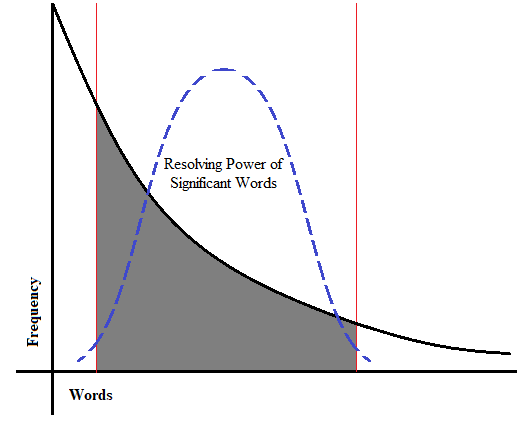
\includegraphics[width=0.6\linewidth]{img/bab2-5.png}
    \caption{Diagram \textit{Word Frequency} [8]}
    \label{fig:2-5}
\end{figure}

Hal yang menjadi sebagai kata kunci dalam penerapan metode otomatis untuk membuat abstrak literatur menggunakan mesin pemrosesan data adalah kata-kata yang paling relevan dan penting dalam artikel yang sedang dianalisis. Kata-kata ini biasanya dipilih berdasarkan topik atau subjek dari artikel tersebut. Dalam \textit{common words} seperti \textit{pronouns}, \textit{prepositions}, dan \textit{articles} dihapus dari daftar kata-kata yang dianalisis karena kata-kata ini tidak memberikan informasi yang signifikan tentang topik atau subjek dari artikel. Sebaliknya, kata-kata yang lebih spesifik dan relevan seperti kata benda dan kata kerja digunakan sebagai kata kunci untuk memilih kalimat-kalimat kunci dalam artikel yang akan digunakan untuk membuat abstrak.

Terdapat penelitian yang dilakukan oleh Rahmah et al \cite{rahmah_critical_2022} dalam menerapkan teori Luhn, dengan Hukum Zipf yang menyatakan bahwa frekuensi kemunculan sebuah kata dalam teks berbanding terbalik dengan peringkatnya dalam daftar frekuensi kata. Dalam konteks pembuatan abstrak otomatis, hukum Zipf dapat digunakan untuk memilih kata-kata kunci yang paling relevan dan penting dalam artikel yang sedang dianalisis. Selain itu, juga membahas tentang skema Bradford \cite{luhn_automatic_1958}, yang merupakan metode untuk mengelompokkan jurnal-jurnal ilmiah berdasarkan topik atau subjek yang sama, dengan adanya \textit{lower cut} dan \textit{upper cut} akan dipilih kata-kata yang diseleksi sebagai tema atau konsep yang dicari sebagaimana yang ditunjukkan pada Gambar \ref{fig:2-5} \cite{luhn_automatic_1958}. Metode tersebut digunakan untuk membantu pembaca literatur teknis menemukan jurnal-jurnal yang relevan dengan topik atau subjek yang sedang mereka teliti \cite{rahmah_critical_2022}.
\DeactivateBG{}

\includepdf{Etc/pemisah.pdf}
\ActivateBG{}
\chapter{METODE PENELITIAN}
\label{BAB3:Metode}

\lipsum[3-4] % generate dummy sentences
\DeactivateBG{}

\includepdf{Etc/pemisah.pdf}
\ActivateBG{}
\chapter{HASIL DAN PEMBAHASAN}
\label{BAB4:hasil}

\section{\textit{Text Preprocessing}}

Data yang telah dikumpulkan berupa 333 dokumen dengan abstrak, pada penelitian ini akan dipakai sehingga berisi 333 baris. Setelah itu, dilakukan suatu \textit{text preprocessing} pada teks tersebut. Pada setelah langkah \textit{text preprocessing} teks tersebut, akan dibagi menjadi dua alur sebagaimana yang telah digambarkan pada Gambar \ref{fig:3-3}, yang pertama ialah sebelum dilakukan suatu pengelompokkan abstrak serupa menjadi klaster dan yang alur lainnya sebelum dilakukan pemilihan kata dasar untuk mencari kata kunci yang relevan dengan teori Luhn.

Adapun tahapan dalam \textit{text preprocessing} hingga mendapatkan hasil berupa kata kunci yang dicari digambarkan pada gambar di bawah ini:
\begin{figure}[H]
    \centering
    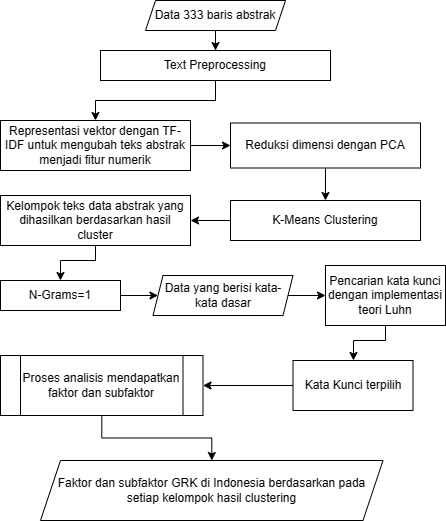
\includegraphics[width=0.75\linewidth]{img/bab4-1.png}
    \caption{Proses tahapan \textit{text preprocessing} hingga hasil menggunakan data studi literatur}
    \label{fig:4-1}
\end{figure}

Di bawah ini, merupakan teknik berupa istilah yang digunakan pada saat melakukan \textit{text preprocessing} sebagai berikut:
\begin{enumerate}
    \item \textit{Lowercase}: Membuat semua teks pada data tersebut menjadi bukan huruf kapital.
    \item \textit{Punctuation}: Menghapus semua unsur tanda baca.
    \item \textit{Stopword}: Menghapus unsur kata-kata yang tidak bermakna, seperti '\textit{is, a, it, in, he, is}'.
    % \item \textit{Alphabet}: Memilih unsur kata-kata yang hanya terdiri dari serangkaian huruf saja.
    \item N-Grams=1 (Unigram): Mendapatkan data yang berisi dari kumpulan kata-kata dasar.
    \item \textit{len(word) $>$ 2}: Mendapatkan kata-kata yang memiliki jumlah huruf lebih dari dua.
    \item \textit{Lemmatization}: Memilih satu dari setiap kata dasar yang memiliki bentuk lema yang sama, seperti terdapat kata '\textit{organizing}' dan '\textit{organize}', maka akan dipilih '\textit{organize}'.
    \item \textit{No Verb}: Menghapus unsur teks yang mengandung kata kerja.
    \item \textit{No Adjective}: Menghapus unsur teks yang mengandung kata sifat.
    \item \textit{No Adposition}: Menghapus unsur teks yang mengandung kata kata depan atau kata sambung.
    \item \textit{No Auxiliary Verb}: Menghapus unsur teks yang mengandung kata kerja bantu.
    \item \textit{No Adverb}: Menghapus unsur teks yang mengandung kata keterangan.
    \item \textit{No Geopolitical Entities} (GPE): Menghapus semua unsur teks yang mengandung unsur nama-nama negara, kota, atau wilayah.
    \item \textit{No Numeric}: Menghapus kata-kata yang memiliki unsur angka saja.
    \item \textit{No Whitespace}: Menghapus unsur yang hanya berisi kata spasi.
\end{enumerate}

\section{Hasil Pengelompokkan Kata Kunci berdasarkan teknik \textit{clustering}}
Pada tahapan awal, data berupa 333 abstrak tersebut dilakukan \textit{preprocessing text}. Kemudian, data yang telah didapatkan tersebut diproses menjadi representasi numerik dari teks abstrak menggunakan metode TF-IDF. TF-IDF digunakan untuk menghitung bobot kata-kata dalam setiap abstrak berdasarkan frekuensi kemunculan kata tersebut di abstrak tertentu dan juga frekuensi kemunculan kata tersebut di semua abstrak. Dengan menggunakan \textit{TfidfVectorizer}, teks abstrak dikonversi menjadi representasi vektor TF-IDF dengan memperhitungkan bobot kata dalam setiap abstrak.

Setelah representasi TF-IDF dibuat, langkah selanjutnya adalah melakukan reduksi dimensi menggunakan PCA. PCA digunakan untuk mengurangi dimensi vektor TF-IDF menjadi dimensi yang lebih rendah, sehingga memungkinkan untuk memvisualisasikan data dalam ruang dua atau tiga dimensi. 

Misalnya, terdapat sejumlah fitur yang direpresentasikan sebagai vektor TF-IDF dari teks. Fitur-fitur ini menggambarkan kata-kata dalam abstrak sebagai dimensi dalam ruang vektor. Jika terdapat 4277 kata unik yang dianggap sebagai fitur, maka akan ada 4277 dimensi dalam vektor tersebut.

Kemudian, metode PCA diterapkan untuk mereduksi dimensi-fitur ini. Dalam tahapan sebelumnya, mengakibatkan dimensi ruang vektor dengan 4277 fitur direduksi menjadi hanya 2 komponen utama. Praktiknya, guna mencari dua sumbu utama yang paling mewakili variasi dalam data. Ketika mereduksi dimensi dari 4277 fitur menjadi 2 komponen, sebagian informasi akan hilang. Persentase \textit{variance} yang dijelaskan oleh dua komponen ini akan mengukur besarnya informasi yang tetap dipertahankan. 

Dalam perhitungan yang didapatkan, komponen pertama memiliki \textit{variance explained ratio} sekitar 0.0235, yang berarti sekitar 2.35\% variasi dalam data oleh komponen ini dan komponen kedua memiliki \textit{variance explained ratio} sekitar 0.0204, yang berarti sekitar 2.04\% variasi dalam data dijelaskan oleh komponen ini. Jumlah dari kedua nilai ini adalah sekitar 4.39\% sebagai informasi dalam data yang berhasil dipertahankan. Dikarenakan pada penerapannya hanya untuk mereduksi dimensi, informasi yang dipertahankan tersebut tidak akan diterapkan sebagai indikator suatu implementasi pada tahapan mendapatkan kata kunci yang dihasilkan di akhir nanti. 

Kembali dalam implementasinya, digunakan \textit{PCA(n\_components=2)} untuk mengambil dua komponen utama dan memvisualisasikan datanya dalam ruang dua dimensi. Komponen utama 1 dan komponen utama 2 pada klasterisasi dengan K-Means merujuk pada hasil reduksi dimensi menggunakan teknik Principal Component Analysis (PCA). Jika nilai komponen utama 1 (nilai x) positif, itu berarti abstrak tersebut cenderung memiliki kontribusi positif dari fitur-fitur yang berkaitan dengan komponen utama 1 tersebut. Sebaliknya, jika nilai komponen utama 1 (nilai x) negatif, itu berarti abstrak tersebut cenderung memiliki kontribusi negatif dari fitur-fitur yang berkaitan dengan komponen utama 1 tersebut.

\begin{figure}[H]
    \centering
    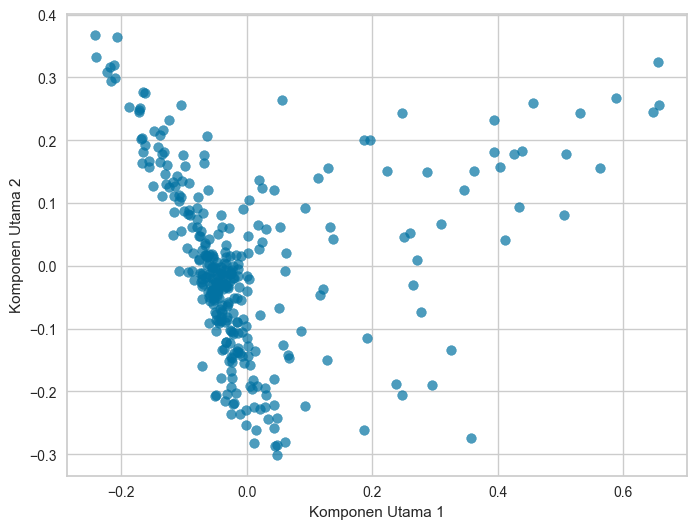
\includegraphics[width=0.7\linewidth]{img/4-221.png}
    \caption{Visualisasi hasil dari PCA}
    \label{fig:4-221}
\end{figure}

Setelah visualisasi PCA, langkah selanjutnya adalah melakukan K-Means \textit{clustering} untuk mengelompokkan abstrak menjadi beberapa klaster berdasarkan fitur TF-IDF yang telah direduksi menggunakan PCA. Pada implementasi KMeans, dibutuhkan satu parameter yaitu nilai dari K. Untuk menentukan nilai K atau jumlah \textit{num\_clusters} yang optimal, dilakukan pencarian dengan menampilkan \textit{Elbow Plot} menggunakan K-Means, dengan uji coba rentang klaster 1-10.

\begin{figure}[H]
    \centering
    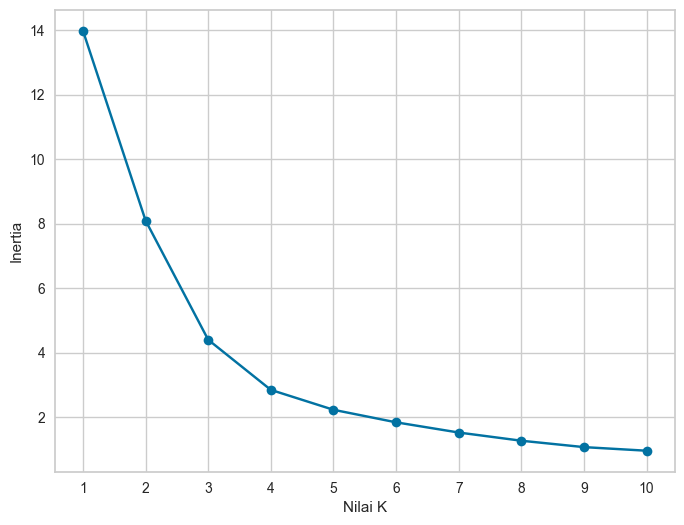
\includegraphics[width=0.725\linewidth]{img/4-21.png}
    \caption{\textit{Elbow Plot} untuk menentukan nilai klaster dengan K-Means}
    \label{fig:4-21}
\end{figure}

Dalam mempermudah penentuan nilai K yang optimum, dilakukan beberapa metrik evaluasi dengan \textit{Davies-Bouldin index} dan \textit{library ElbowVisualizer}, kedua metrik evaluasi tersebut digunakan untuk mengevaluasi nilai K yang optimal dalam algoritma K-Means. \textit{Davies-Bouldin index} mengukur kualitas pembagian klaster berdasarkan jarak antara klaster yang berdekatan dan dispersi internal setiap klaster \cite{sanghun2022}. Semakin rendah nilai \textit{Davies-Bouldin index}, semakin baik pembagian klaster dan semakin optimal nilai K yang digunakan. Selain itu, dengan \textit{library ElbowVisualizer} untuk membantu dan memperjelas dari visualisasi \textit{Elbow Plot}, pada saat titik di nilai \textit{inertia} mulai menurun secara lambat atau berhenti menurun drastis, itulah titik yang disarankan sebagai jumlah klaster yang optimal. Hasil dari kedua evaluasi tersebut menunjukkan nilai K=4 yang merupakan nilai K yang optimal, sehingga diterapkan fungsinya yakni \textit{KMeans(n\_clusters=4)}.

\begin{figure}[H]
    \centering
    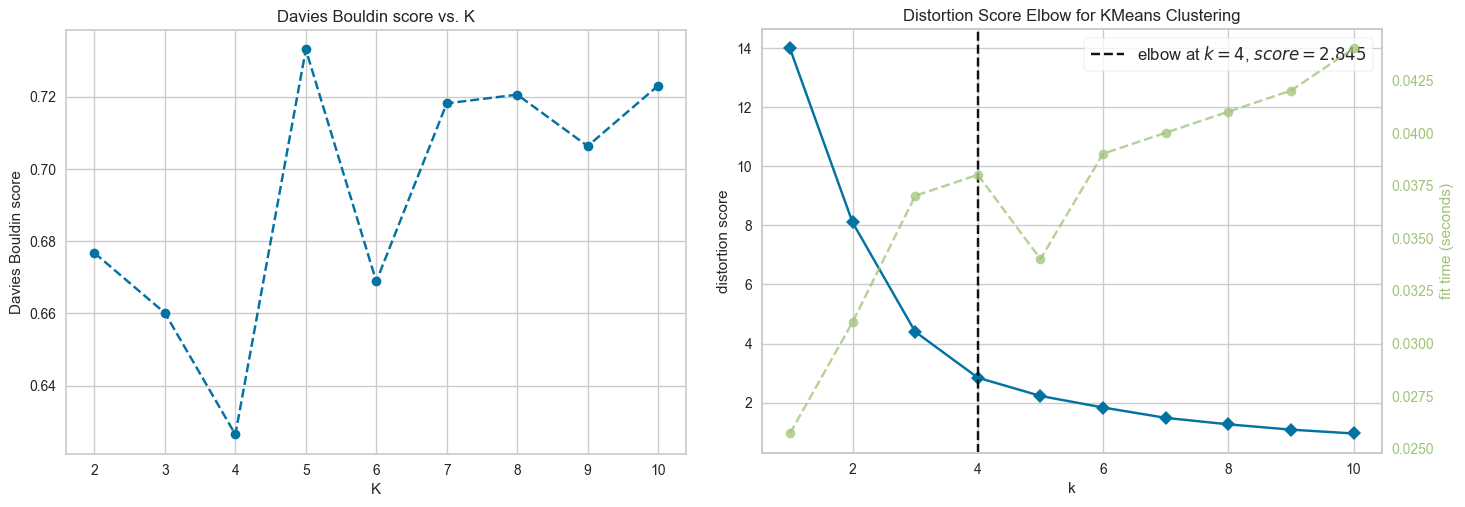
\includegraphics[width=0.9\linewidth]{img/4-21-3.png}
    \caption{Metrik Evaluasi nilai K dengan \textit{Davies-Bouldin index} dan \textit{library ElbowVisualizer}}
    \label{fig:4-21-3}
\end{figure}

Setelah melakukan K-Means \textit{clustering} dan menentukan jumlah klaster yang optimal berdasarkan \textit{elbow plot} dengan didukung validasi berupa evaluasi metrik, selanjutnya dapat diketahui dalam setiap klaster dengan menggunakan atribut dari objek K-Means untuk menyimpan label klaster pada setiap sampel data abstrak dan mengelompokkannya berdasarkan warna yang berbeda. 

Dalam konteks klasterisasi perwarnaan dengan K-Means, komponen utama 1 dan komponen utama 2 adalah dua dimensi baru yang dihasilkan dari PCA. Setiap baris data dalam dataset asli direpresentasikan oleh dua nilai pada komponen utama 1 dan komponen utama 2. Nilai-nilai ini menggambarkan lokasi relatif data dalam ruang dua dimensi yang telah direduksi. Pada saat PCA telah dilakukan, visualisasi data abstrak dalam ruang dua dimensi dengan \textit{scatter plot} menunjukkan bahwa setiap titik pada \textit{scatter plot} merepresentasikan satu abstrak, dan dapat dilihat berupa pola dan struktur data sebelum melakukan \textit{clustering}. 

\begin{figure}[H]
    \centering
    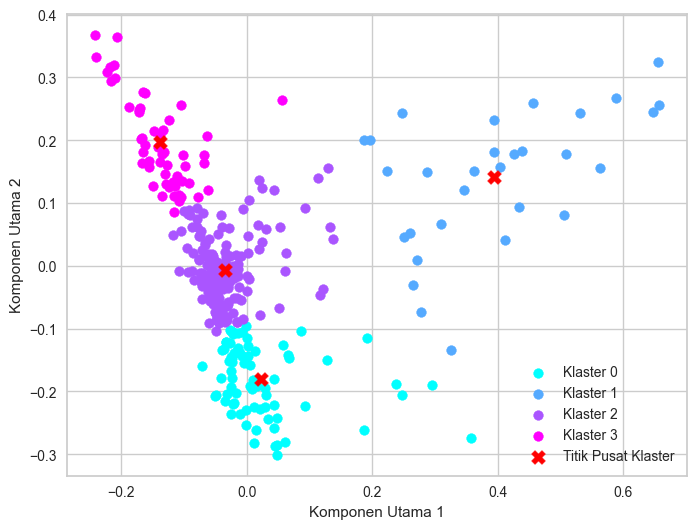
\includegraphics[width=0.7\linewidth]{img/4-222.png}
    \caption{Klasterisasi Pewarnaan dengan K-Means}
    \label{fig:4-222}
\end{figure}

% Selain itu, untuk mempermudah dalam melihat klaster mana yang lebih baik, dilakukanlah \textit{Silhouette plot} yang merupakan metode untuk mengukur seberapa baik setiap data abstrak dikelompokkan oleh K-Means. Plot ini menunjukkan nilai \textit{silhouette score} untuk setiap titik klaster pada data abstrak, nilai \textit{silhouette score} mengukur seberapa mirip data abstrak dengan kelompoknya sendiri dibandingkan dengan kelompok lain. \textit{Silhouette plot} juga membantu mengidentifikasi apakah ada kelompok yang tidak terdefinisi dengan baik atau apakah data abstrak tergolong dalam kelompok yang sesuai.

% \begin{figure}[H]
%     \centering
%     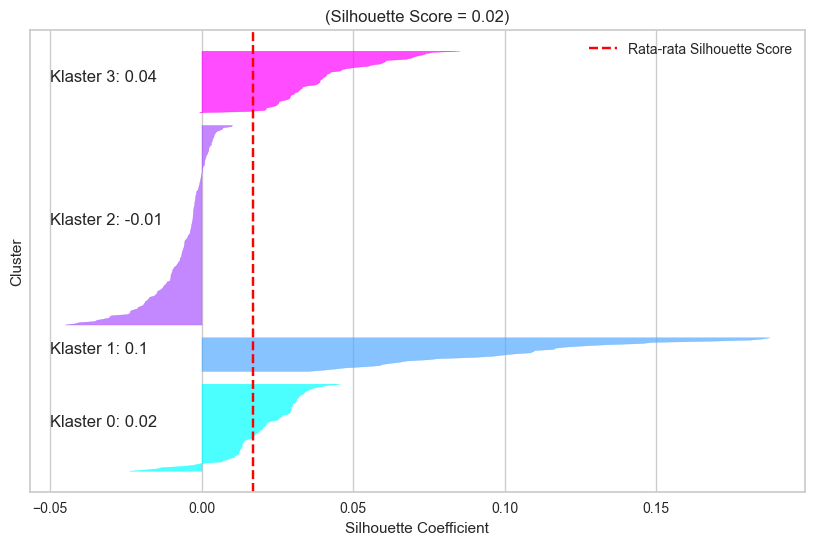
\includegraphics[width=0.7\linewidth]{img/4-23.png}
%     \caption{\textit{Silhouette Plot} untuk K-Means \textit{Clustering}}
%     \label{fig:4-23}
% \end{figure}

% Dari hasil tersebut, terdapat klaster yang memiliki warna yang menjulang jauh melebihi rata-rata dari \textit{Silhouette Score} yang telah didapatkan senilai 0.03 tersebut, yang menandakan bahwa klaster tersebut memiliki \textit{Silhouette Coefficient} yang tinggi dibandingkan dengan klaster lainnya. Klaster dengan \textit{Silhouette Coefficient} yang tinggi menunjukkan bahwa titik-titik data dalam klaster tersebut lebih dekat satu sama lain dan lebih terpisah dari titik-titik data di klaster lain. Hal ini, menunjukkan klaster tersebut memiliki titik-titik data yang sangat serupa dan kohesif. Dalam konteks analisis \textit{clustering}, hal ini dapat diartikan sebagai kelompok yang lebih homogen atau memiliki karakteristik yang sama. 

Pada keempat kluster yang berisi kelompok-kelompok abstrak tersebut, akan dipakai pada tahap selanjutnya, yaitu dilakukan penyeleksian dengan prinsip teori Luhn yang hasilnya nanti akan diterapkan suatu \textit{keyword extraction} untuk menentukan kata-kata kunci yang paling relevan dalam setiap klaster sebagai faktor dan sub-faktor GRK. 

\section{Hasil Pemilihan Kata Kunci berdasarkan Teori Luhn}
Pada tahapan memilih kata kunci, berdasarkan teori Luhn, data yang telah didapatkan dari hasil klasterisasi setiap kelompok, dilakukan suatu pemecahan kata-kata dasar pada masing-masing klaster dengan N-Grams = 1 (Unigram). 

\begin{table}[H]
\centering
\caption{Total jumlah kata setiap klaster}
\label{tab:jumlah_kata}
\resizebox{0.35\columnwidth}{!}{%
\begin{tabular}{l|c}
\hline
\textbf{Klaster} & \textbf{Total Jumlah Kata} \\
\hline
\textit{Cluster 0} & \textit{13198 Kata} \\
\textit{Cluster 1} & \textit{8137 Kata} \\
\textit{Cluster 2} & \textit{2473 Kata} \\
\textit{Cluster 3} & \textit{6476 Kata} \\
\hline
\end{tabular}%
}
\end{table}


Setelah dilakukan proses pemecahan menjadi kata-kata dasar pada setiap klaster, didapatkan jumlah kata yang didapatkan sebagaimana yang telah ditunjukkan pada Tabel \ref{tab:jumlah_kata}. Kemudian untuk melihat suatu frekuensi dari masing-masing kata dasar, terdapat visualisasi dengan \textit{Word cloud} untuk menunjukkan representasi visual dari data teks yang menggambarkan frekuensi kata-kata dalam teks tersebut \cite{hicke_word_2022}. Dalam \textit{word cloud}, kata-kata yang muncul lebih sering akan ditampilkan dengan ukuran yang lebih besar, sedangkan kata-kata yang muncul lebih jarang akan ditampilkan dengan ukuran yang lebih kecil. 

\begin{figure}[H]
    \centering
    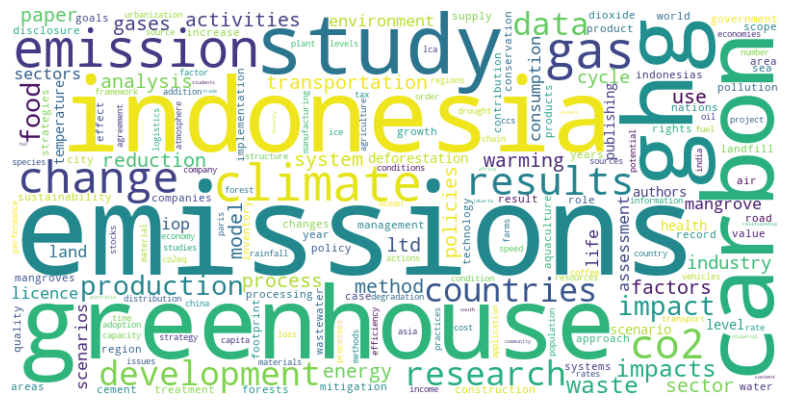
\includegraphics[width=0.6\linewidth]{img/4-31-1.png}
    \caption{Representasi visual frekuensi data dengan \textit{word cloud} pada \textit{Cluster 0}}
    \label{fig:4-31-1}
\end{figure}
\begin{figure}[H]
    \centering
    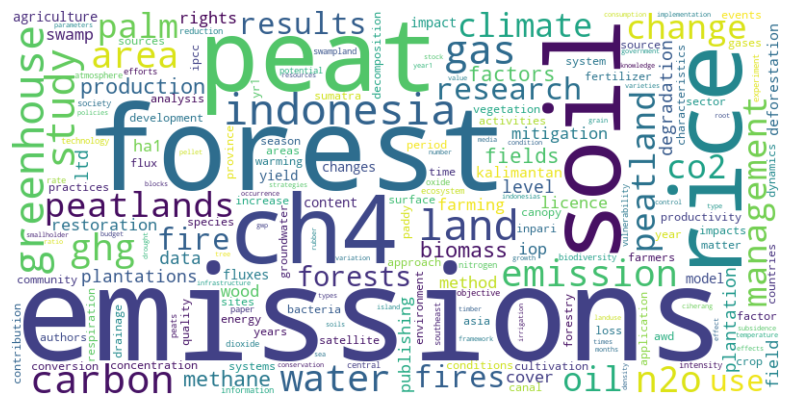
\includegraphics[width=0.6\linewidth]{img/4-31-2.png}
    \caption{Representasi visual frekuensi data dengan \textit{word cloud} pada \textit{Cluster 1}}
    \label{fig:4-31-2}
\end{figure}
\begin{figure}[H]
    \centering
    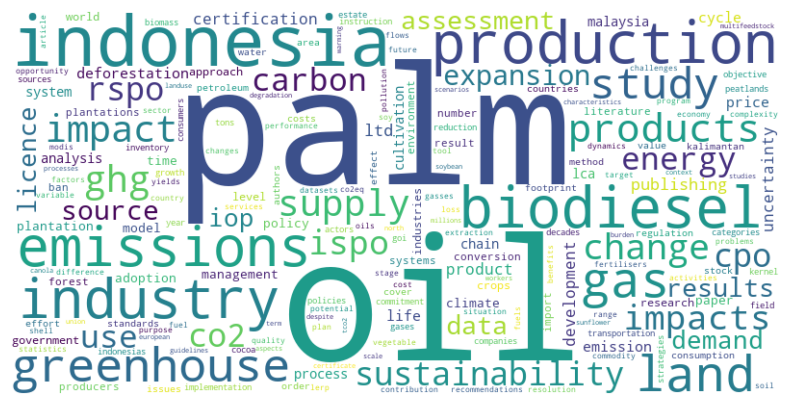
\includegraphics[width=0.6\linewidth]{img/4-31-3.png}
    \caption{Representasi visual frekuensi data dengan \textit{word cloud} pada \textit{Cluster 2}}
    \label{fig:4-31-3}
\end{figure}
\begin{figure}[H]
    \centering
    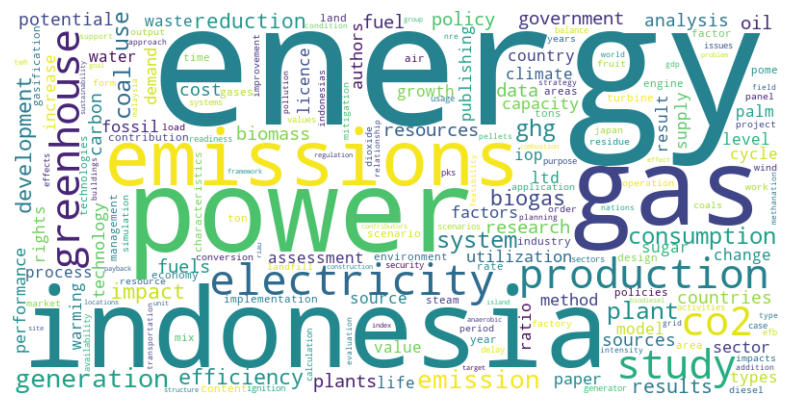
\includegraphics[width=0.6\linewidth]{img/4-31-4.png}
    \caption{Representasi visual frekuensi data dengan \textit{word cloud} pada \textit{Cluster 3}}
    \label{fig:4-31-4}
\end{figure}

Pada keempat representasi visual menggunakan \textit{word cloud} sebelumnya, bisa dilihat bahwa masing-masing setiap klaster memiliki unsur kata dengan jumlah frekuensi yang cukup sedikit berbeda. Terlihat pula kata-kata dasar apa yang memiliki ukuran paling besar dan yang kecil. Namun, pada tahapan seleksi teori Luhn ini bukanlah memilih kata-kata yang memiliki frekuensi terbesar, melainkan semua data dengan jumlah frekuensi kata pada setiap klaster yang akan dipakai pada tahapan teori Luhn. Adapun bagian-bagian kata yang memiliki frekuensi terbesar dan frekuensi terkecil akan dibuang, karena berdasarkan teori Luhn, interval data pada rentang tersebut merupakan istilah-istilah yang kurang baik dalam memilih kata kunci yang relevan secara optimal.

Berikut adalah langkah-langkah dalam pemilihan kata-kata dari hasil \textit{clustering} dan penerapan teori Luhn, serta \textit{labelling} faktor dan subfaktor pada setiap klasternya sebagai berikut:

\begin{enumerate}
    \item Pemisahan Kalimat Abstrak menjadi Kata-Kata Dasar: Pada setiap klaster, semua kalimat abstrak akan dipecah menjadi kata-kata dasar. Hal tersebut membantu mengidentifikasi kata-kata kunci yang paling mewakili konten dari setiap klaster.
    \item Perhitungan Frekuensi Kemunculan Kata: Frekuensi kemunculan setiap kata dalam klaster dihitung. Dengan informasi ini, didapatkan gambaran tentang kata-kata yang paling sering muncul dalam konteks klaster tertentu.
    \item Penerapan Teori Luhn: Prinsip teori Luhn digunakan untuk memilih kata-kata yang memiliki frekuensi kemunculan di dalam interval yang ditentukan. Interval ini mengarahkan untuk menghilangkan beberapa kata yang mungkin terlalu umum atau terlalu jarang muncul. Tujuannya adalah mendapatkan kata-kata kunci yang lebih relevan.
    \item Penentuan Batas: Berdasarkan teori Luhn, batas interval ditentukan. Batas ini mencakup lower cut (batas bawah) dan upper cut (batas atas). Kata-kata kunci yang masuk dalam interval ini memiliki potensi sebagai representasi yang tepat dari faktor penyebab GRK.
    \item Seleksi Kata-Kata Kunci: Kata-kata kunci yang memiliki frekuensi kemunculan di dalam interval batas akan dipilih. Ini menghasilkan kumpulan kata-kata kunci yang akan mewakili konten klaster tertentu.
    \item Analisis Kualitatif: Setelah kata-kata kunci dipilih, dilakukan analisis kualitatif lebih lanjut secara manual. Setiap kata kunci akan ditafsirkan dalam konteks faktor penyebab Gas Rumah Kaca (GRK). Hal ini melibatkan pemahaman mendalam tentang makna kata-kata, serta bagaimana kata-kata tersebut terkait dengan aspek GRK.
    \item \textit{Labelling} Faktor dan Subfaktor: Setelah analisis kualitatif, kata-kata kunci tersebut dapat digunakan sebagai label untuk mengidentifikasi faktor dan subfaktor GRK dalam setiap klaster. Label ini memberikan representasi komprehensif tentang apa yang mendasari peningkatan GRK.
\end{enumerate}

Setelah melakukan langkah-langkah tersebut pada setiap klaster, maka didapatkanlah faktor dan sub-faktor GRK yang relevan dengan menggunakan kata-kata kunci yang telah dipilih. Proses ini juga merupakan interpretasi akhir mengenai aspek atau faktor penyebab GRK dalam masing-masing konteks klaster.

\section{Hasil Interpretasi Kata Kunci Berdasarkan Teknik \textit{Clustering} dan Seleksi Teori Luhn}

\begin{table}[H]
\centering
\caption{Hasil Kata Kunci yang Terpilih berdasarkan teknik Clustering dan implementasi teori Luhn}
\label{tab:factors}
\resizebox{0.95\columnwidth}{!}{%
\begin{tabular}{|l|l|p{0.95\textwidth}|}
\hline
\multicolumn{3}{|c|}{\textbf{Faktor dan 10 Subfaktor Aspek GRK di Indonesia berdasarkan Kata Kunci yang Dihasilkan}} \\ \hline
\textbf{Klaster} & \textbf{Faktor} & \textbf{Subfaktor} \\ \hline
\textit{Cluster 0} & \textit{Deforestation} & \textit{emissions peat, deforestation degradation, mangrove deforestation, mangrove carbon, deforestation mangroves, emissions peatlands, vegetation indices, land fires, emissions peat, forestry land} \\ \hline
\textit{Cluster 1} & \textit{Biodiesel} & \textit{biodiesel production, biomass indonesia, indonesias palm, palm peatlands, biodiesel palm, palm oil, impacts biodiesel, footprint biodiesel, palm expansion, biofuel role} \\ \hline
\textit{Cluster 2} & \textit{co2 / Carbon} & \textit{buildings co2emissions, co2 cement, co2resistant cementing, coal power, waste composition, co2 atmosphere, dependence fuels, contributors carbon, waste business, pollutants countries} \\ \hline
\textit{Cluster 3} & \textit{Electricity} & \textit{electricity consumption, policies energy, buildings energy, boiler efficiency, electricity supply, energy policy, generator efficiency, indonesian electricity, energy sources, capacity biogas} \\ \hline
\end{tabular}%
}
\end{table}



% \begin{table}[H]
% \caption{Hasil Kata Kunci yang Terpilih Berdasarkan Teknik \textit{Clustering} dan Implementasi Teori Luhn}
% \label{tab:kata_kunci_terpilih}
% \resizebox{\columnwidth}{!}{%
% \begin{tabular}{@{}|l|p{0.8\textwidth}|@{}}
% \midrule
% \multicolumn{3}{c}{\textbf{Faktor dan 10 Subfaktor Aspek GRK di Indonesia berdasarkan Kata Kunci yang Dihasilkan }}                                        \\ \midrule
% \textit{\textbf{Cluster 0}} & \textit{Deforestation} & \textit{emissions peat, eforestation degradation, mangrove deforestation, mangrove carbon, deforestation mangroves, emissions peatlands, vegetation indices, land fires, emissions peat, forestry land}                                                        \\ \midrule
% \textit{\textbf{Cluster 1}}          & \textit{emissions, forest, soil, peat, rice, ch4, indonesia, greenhouse, land, gas, study, carbon, water, ghg, n2o, emission, area, peatlands, management, palm}                                                    \\ \midrule
% \textit{\textbf{Cluster 2}}          & \textit{oil, palm, emissions, indonesia, production, gas, greenhouse, biodiesel, industry, ghg, study, soil, land, forest, peat, plantations, n2o, carbon, co2, impact}                                                                            \\ \midrule
% \textit{\textbf{Cluster 3}}          & \textit{energy, power, indonesia, gas, emissions, electricity, production, greenhouse, co2, study, generation, emission, plant, consumption, ghg, coal, system, use, biogas, efficiency}                                                               \\  \bottomrule
% \end{tabular}%
% }
% \end{table}

% \begin{itemize}
    % \item [a.] \textbf{\textit{Cluster 0}}: \textit{emissions, indonesia, greenhouse, carbon, ghg, study, emission, gas, climate, change, co2, results, development, research, countries, data, production, impact, food, impacts}
    % \item [b.] \textbf{\textit{Cluster 1}}: \textit{emissions, forest, soil, peat, rice, ch4, indonesia, greenhouse, land, gas, study, carbon, water, ghg, n2o, emission, area, peatlands, management, palm}
    % \item [c.] \textbf{\textit{Cluster 2}}: \textit{oil, palm, indonesia, production, biodiesel, emissions, industry, gas, land, greenhouse, study, products, impact, supply, ghg, change, impacts, ispo, cpo, rspo}
    % \item [d.] \textbf{\textit{Cluster 3}}: \textit{energy, power, indonesia, gas, emissions, electricity, production, greenhouse, co2, study, generation, emission, plant, consumption, ghg, coal, system, use, biogas, efficiency}
% \end{itemize}

Setelah dilakukan suatu pemilihan kata-kata kunci dari gabungan hasil proses teknik \textit{clustering} dan prinsip teori Luhn tersebut, berdasarkan sumber dari data studi literatur, aspek dan faktor penyebab dari GRK yang ada di Indonesia, maka dari hasil tersebut bisa dijadikan sebagai landasan secara efektif untuk melihat kondisi saat ini dengan memanfaatkan studi literatur 5 tahun terakhir yang membahas terkait subjek atau urgensi perihal GRK di Indonesia. 

Contohnya seperti \textit{emissions peat, deforestation degradation, mangrove deforestation} yang merupakan subfaktor dari faktor \textit{deforestation} dan faktor klaster lainnya yang memiliki keterkaitan antara sesama kata-kata kunci yang bisa digabungkan menjadi frasa berupa subfaktor seperti contoh tersebut. Oleh karena itu, dari hasil penelitian ini, dari kata-kata kunci yang didapatkan, dapat diketahui faktor dan subfaktor atau bahkan aspek hal lainnya yang bisa menjadi perhatian bahwa dengan memanfaatkan teknologi saat ini seperti \textit{Artificial Intellegence} dan juga analisis data yang didukung juga berdasarkan teori, dapat membantu dalam analisis tersebut, terutama dalam mengetahui hal-hal yang berhubungan dengan aspek yang dicari.
\DeactivateBG{}

\includepdf{Etc/pemisah.pdf}
\ActivateBG{}
\chapter{KESIMPULAN DAN SARAN}
\label{BAB5:kesimpulan}

\section{Kesimpulan}
Dari hasil analisis data teks menggunakan pengolahan dan teknik dengan \textit{text mining}, \textit{clustering}, dan penyeleksian menggunakan teori Luhn pada data abstrak dari studi literatur lima tahun terakhir, telah didapatkan faktor dan subfaktor kata-kata kunci yang memiliki relevan sebagai faktor penyebab Gas Rumah Kaca (GRK) di Indonesia berupa empat kelompok, yaitu \textit{deforestation, biodiesel, co2/carbon, electricity}. Hasil analisis ini dapat memberikan informasi yang bermanfaat terkait permasalahan GRK saat ini dan dapat menjadi landasan untuk langkah-langkah penanganan dan mitigasi lebih lanjut terhadap dampak GRK di Indonesia terutama pada beberapa aspek yang telah dihasilkan dari keempat kelompok hasil \textit{clustering} sebelumnya.

\section{Saran}
Untuk penelitian selanjutnya, disarankan agar dapat memperluas sumber data studi literatur dengan mencakup lebih banyak publikasi terkini dan diversifikasi sumber literatur, termasuk jurnal ilmiah, laporan pemerintah, dan publikasi akademis lainnya. Penggunaan sumber data yang lebih luas akan memberikan gambaran yang lebih komprehensif terkait faktor penyebab GRK di Indonesia.

Selanjutnya, direkomendasikan untuk melanjutkan penelitian dengan kolaborasi para ahli dalam membantu memvalidasi apa yang telah dihasilkan pada penelitian di bidang terkait. Selain itu, dalam upaya meningkatkan pemahaman yang lebih holistik pada aspek dampak GRK di Indonesia, disarankan untuk dilakukan kajian lebih lanjut dengan mempertimbangkan aspek waktu, geografis, dan perubahan iklim, sehingga dapat memberikan pemahaman yang lebih holistik mengenai dampak GRK di Indonesia yang lebih signifikan dalam pengembangan strategi dan kebijakan mitigasi GRK yang efektif serta berkelanjutan di Indonesia. 
\DeactivateBG{}

\includepdf{Etc/pemisah.pdf}
\ActivateBG{}

%------------------------------------------------------------
% BIBLIOGRAPHY 
%------------------------------------------------------------
\begin{singlespace}
  \bibliographystyle{apalike}
  \addcontentsline{toc}{chapter}{DAFTAR PUSTAKA}
  \bibliography{referensi}
\end{singlespace}

\DeactivateBG{}

\includepdf{Etc/pemisah.pdf}
\ActivateBG{}

%------------------------------------------------------------
% Appendices
% (comment) uncomment kode di bawah ini untuk (tidak) menggunakan lampiran
% tambahkan sendiri folder-folder (lampiran) yang lain
%------------------------------------------------------------
\appendix
\Appendix{Judul Lampiran 1}
\label{lampiran1}

\lipsum[1] % generate dummy sentences

\begin{myblock}{Cara \textit{Web Scraping}}\label{Lampiran1}
\begin{minted}[xleftmargin=20pt,linenos]{python}

from bs4 import BeautifulSoup
import requests
from time import sleep
base_url = "https://www.oreilly.com/search/" + \
           "/?q=data&type=*&rows=10&page="


books = []
NUM_PAGES = 31

for page_num in range(1, NUM_PAGES + 1):
    print("souping page", page_num, ",", len(books), " found")
    url = base_url + str(page_num)
    soup = BeautifulSoup(requests.get(url).text, 'html5lib')
    
    for td in soup('td', 'thumbtext'): if not is_video(td):
        books.append(book_info(td))
        
    # give a break
    sleep(30)

def get_year(book):
    return int(book["date"].split()[1])

year_counts = Counter(get_year(book) for book in books 
                       if get_year(book) <= 2014)

import matplotlib.pyplot as plt
years = sorted(year_counts)
book_counts = [year_counts[year] for year in years] 
plt.plot(years, book_counts)
plt.ylabel("# of data books")
plt.title("Data is Big!")
plt.show()

\end{minted}
\end{myblock}


% \Appendix{Judul Lampiran 2}
\label{lampiran2}

\lipsum[2-3] % generate dummy sentences

\backmatter

\end{document}

%--------------------- end of file ---------------------------------------